\documentclass{article}
\usepackage[utf8]{inputenc}
\usepackage{amsmath, amssymb}
\usepackage[margin=1.0in]{geometry}
\usepackage{graphicx}
\usepackage{mathrsfs}
\usepackage{hyperref}
\usepackage{float}
\usepackage{subcaption}

\title{Note of Fast Runner}
\author{Ken}
\date{June, 2018\footnote{Last update: \today}}

\usepackage{natbib}
\usepackage{graphicx}
\graphicspath{ {./images/} }
\usepackage{amsthm}


\newtheorem{prop}{Proposition}

\begin{document}

\maketitle

\section{About systems and methods}
\subsection{Requirements - system}
\begin{itemize}
\item List of assumptions
\item Capture the required parameters (i.e. how to normalize the systems)
	\begin{itemize}
	\item Resonance
	\item Nonlinear elastic components
	\begin{itemize}
	\item a set of linear components for multiple modes? 
	\end{itemize}
	\end{itemize}
	
\item 
\end{itemize}
\subsection{Requirements - method}
\begin{itemize}
\item Applicable to complex system (e.g. for the designed mechanism)
\item Nondimensionlization (so that it can be used for robots with different scales)
\item Stability analysis
\item Robustness
\end{itemize}

\subsection{Remarks}
\begin{itemize}
\item Impact does not cause velocity change on runner with massless leg!
\item In SCS, to simulate massless leg, it is better to use only one body, and manipulate the relation between the contact point and the body in controller instead.
\end{itemize}

\subsection{ToDo}
\begin{itemize}
\item Rearrange/updating references for fastRunner
\item Check if the foot is sliding
\item Check optimization tools ihmc have
\begin{itemize}
\item parameter optimization tool using Gradient Decent or GA
\end{itemize}
\item Ask Cris about the parameter range/selection
\end{itemize}

\subsection{Questions}
Direction
\begin{itemize}
\item Should I exclude the gyroscopic-based stabilization? 
\item Eigen values of linearized system, Poincare map analysis, anything else I should study for the stability analysis?
\item The linkage between the control in simulation and mechanism design
	\begin{itemize}
	\item Parameters
	\item How to design a mechanism can emulate PD control?
	\end{itemize}
\end{itemize}
General Utilities 
\begin{itemize}
\item Any solver for nonlinear program IHMC used?
\item Any trajectory optimization package IHMC used?
\item Methods to get stable Reciprocating Spoked Runner?
\end{itemize}

Past simulations
\begin{itemize}
\item Why the abstract runner (in spoked runner project) can be stabilized in x direction? 
\begin{figure}[h]
\centering

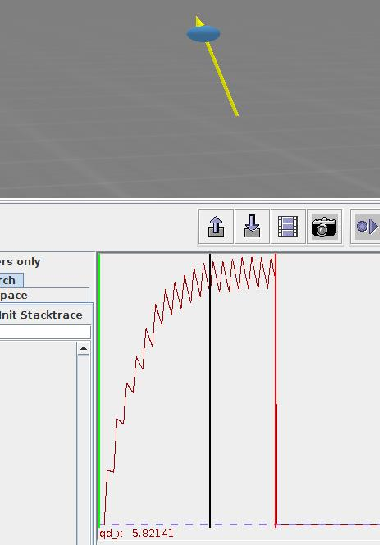
\includegraphics[scale = 0.5]{abstractRunner.pdf} 
\caption{The Abstract Runner}
%\label{fig.1DOF-Hopper}
\end{figure}
\begin{itemize}
\item The simulation setup is really robust for a large set of initial conditions/throttle angles
\item It turns out its because the added \underline{wind resistance} dissipate a lot of energies.
\end{itemize}


\item Methods to get stable Reciprocating Spoked Runner?
\item What is the line \underline{private static final long serialVersionUID } for?

\end{itemize}

\pagebreak
%\clearpage
\section{Pitch Stability of an Vertically Open-loop Hopper}

\subsection{Jorge Cham's Dissertation - openloop control of 1DOF vertical hopper }
\begin{figure}[h]
\centering

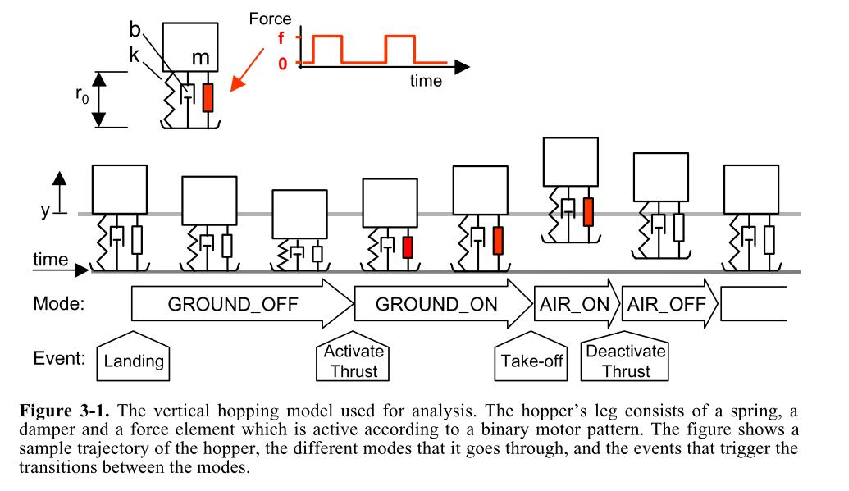
\includegraphics{test.pdf} 
\caption{The schematic of a 1 DOF hopper \cite{Cham2002}}
\label{fig.1DOF-Hopper}
\end{figure}


\subsubsection{Equation of motion}
Using the model as shown in Fig. \ref{fig.1DOF-Hopper}, during the stand phase (i.e. $y\leq 0$), the equation of motion can be expressed as:
\begin{align*}
m \ddot y = -b\dot y +-ky -mg + f
\end{align*}
\noindent where $m$ is the mass, $b$ is the damping, $k$ is the stiffness, $f$ is the control input.
Normalized by weight, the equation becomes
\begin{align*}
 \ddot y = -b/m\dot y +-k/my -g + f/m
\end{align*}

\noindent Expressed in state space form:

\begin{align}
\begin{bmatrix}
\dot y  \\
\ddot y 
\end{bmatrix} = \begin{bmatrix}
0 & 1 \\
-k/m & -b/m
\end{bmatrix}\begin{bmatrix}
 y  \\
\dot y 
\end{bmatrix} + 
\begin{bmatrix}
0  \\
-g+f/m 
\end{bmatrix}
\end{align}
or equivalently
\begin{align}
\label{eq:groundEOM}
\dot X = \begin{bmatrix}
0 & 1 \\
-\omega^2 & -2\xi\omega
\end{bmatrix}X + 
\begin{bmatrix}
0  \\
-g+f_n(t)
\end{bmatrix} &= \begin{bmatrix}
0 & 1 \\
-k_p & -k_d
\end{bmatrix}X + 
\begin{bmatrix}
0  \\
-g+f_n(t)
\end{bmatrix}
\end{align}
where $X \triangleq [y,\dot y]^T$.
When the hopper is in the air (i.e. $y> 0$, flight phase), 
\begin{align}
\label{eq:airEOM}
\dot X = \begin{bmatrix}
0 & 1 \\
0 & 0
\end{bmatrix}X + 
\begin{bmatrix}
0  \\
-g 
\end{bmatrix}
\end{align}
\noindent Define the force  of an open-loop motor pattern
\begin{align}
 f_n(t)=\begin{cases}
    f/m, & \text{if $t_{off}<t<t_{off}+t_{on}$}.\\
    0, & \text{otherwise}.
  \end{cases}
\end{align}

\subsection{Stability Analysis of an Open-loop Controlled Hopper with Discrete Pitch Angle Control}
Use the state space of z motion form \ref{eq:groundEOM} with a simplified open-loop force input:

\begin{align}
\begin{bmatrix}
\dot z  \\
\ddot z 
\end{bmatrix} = \begin{bmatrix}
0 & 1 \\
-kp_z & -kd_z
\end{bmatrix}\begin{bmatrix}
 z  \\
\dot z 
\end{bmatrix} + 
\begin{bmatrix}
0  \\
-g+f_n(t)
\end{bmatrix}
\end{align}
where 
\begin{align}
 f_n(t)=\begin{cases}
    f_n\triangleq f/m, & \text{if $t_{flight}<t<t_{flight}+t_{contact}$}.\\
    0, & \text{otherwise}.
  \end{cases}
\end{align}
To further simplify the problem, assuming $f_n(t)$ is much more dominant than $-kp_zz-kd_z\dot z$-g so that:
\begin{align}
\label{eq:SimpleHopper}
\begin{bmatrix}
\dot z  \\
\ddot z 
\end{bmatrix} \approx \begin{bmatrix}
0 & 1 \\
0 & 0
\end{bmatrix}\begin{bmatrix}
 z  \\
\dot z 
\end{bmatrix} + 
\begin{bmatrix}
0  \\
f_n(t)
\end{bmatrix}
\end{align}
Assumptions:
\begin{itemize}
\item $f_n(t)$\footnote{Conceptually, the $f_n(t)$ can be treated as a force applied from a nonlinear component which connects the massless leg to the body (so there is no velocity change happen at foot strike)} can induce stable vertical hopping motion.
\item $t_0$ starts when the foot leaves the ground.
\item $t_{flight} + t_{contact} = T$, $t_{contact} = \alpha$, and $T>\alpha$
\end{itemize}
Then the pitch dynamics with feedback control can be expressed as:
\begin{align}
\begin{bmatrix}
\dot \theta  \\
\ddot \theta
\end{bmatrix} = \begin{bmatrix}
0 & 1 \\
0 & 0
\end{bmatrix}\begin{bmatrix}
 \theta  \\
\dot \theta
\end{bmatrix} + 
\begin{bmatrix}
0  \\
-f_n(t)m/I\Delta x
\end{bmatrix}
\end{align}
\subsubsection{Poincare Section}
\noindent Denote the state at the $n^{th}$ step Poincare section $\theta_n, \dot \theta_n$ (defined at the start of the flight phase). Then we can calculate the state at Poincare section at the $n+1^{th}$ step:
\begin{align}
\label{eq:PoincareSection1}
\dot \theta_{n+1} &= \dot \theta_{n} - \frac{f}{I}\Delta x t_{contact} \\
\nonumber\theta_{n_{touchDown}} &= \theta_{n} + \dot \theta_{n}t_{flight}\\
\nonumber\dot \theta_{n_{touchDown}} &= \dot \theta_{n}\\
\nonumber\theta_{n+1} &= \theta_{n} + \dot \theta_{n}t_{flight} + \dot \theta_{n}t_{contact} - \frac{1}{2}\frac{f}{I}\Delta xt^2_{contact}\\
\label{eq:PoincareSection2} & = \theta_n + T\dot \theta_n - \frac{1}{2}\frac{f}{I}\alpha^2\Delta x
\end{align}


\subsubsection{Poincare Map of Pitch Dynamics with Proportional Control}
By designing a proportional control such that $\Delta x = k\phi_n$ and defining $K =\frac{1}{2} \frac{f}{I}k$, Eq. \ref{eq:PoincareSection1} and Eq.\ref{eq:PoincareSection2} can be expressed as follows:
\begin{align*}
\theta_{n+1} &= \theta_n  - \alpha^2 K \theta_n + T\dot \theta_n\\
\dot \theta_{n+1} &= \dot \theta_n  - 2\alpha K \theta_n\\
\end{align*}
Arranged them in the state space equation, we can get a discrete map $M$ (i.e. Poincare Map, with set of difference equations):

\begin{align}
\label{eq:PoincareMap}
\begin{bmatrix}
\theta_{n+1}  \\
\dot \theta_{n+1}
\end{bmatrix} = \begin{bmatrix}
1-\alpha^2 K & T \\
-2\alpha K & 1
\end{bmatrix}\begin{bmatrix}
 \theta_n  \\
\dot \theta_n 
\end{bmatrix} = M
\begin{bmatrix}
 \theta_n  \\
\dot \theta_n 
\end{bmatrix}
\end{align}


\noindent \textbf{Eigen value analysis}\\
To analyze the stability of the equation in \ref{eq:PoincareMap}, we need to check whether the eigen values of Poincare map $M$ are within the unit cycle. Similar to the Rooth-Herwitz method for the continuous map, we can use Jury Stability Test (Ogata, 1985)\footnote{contents quotated from \cite{Cham2002}}, which states that a discrete system of two dimensions with the characteristic equations P(z) of the form:
\begin{align*}
P(z) = a_0z^2 + a_1z + a_2
\end{align*}
where $a_0>0$, is stable if the following conditions are all satisfied:
\begin{align*}
|a_2|&<a_0\\
a_0+a_1+a_2&>0\\
a_0-a_1+a_2&>0\\
|(a_0+a_2)(a_2-a_0)|&>|a_1(a_0-a_1)|\\
\end{align*}
For a Jacobian of the form 
\begin{align*}
J = \begin{bmatrix}
J_1 & J_2 \\
J_3 & J_4
\end{bmatrix}
\end{align*}
The characteristics equation can be expressed as follows:
\begin{align*}
P(z) = z^2-(J_1+J_4)z +(J_1J_4-J_2J_3)
\end{align*}
Substituting into the stable conditions stated above,
\begin{align}
\label{eq:condition1}
|(J_1J_4-J_2J_3)|&<1\\
\label{eq:condition2}
1-(J_1+J_4)+(J_1J_4-J_2J_3)&>0\\
\label{eq:condition3}
1+(J_1+J_4)+(J_1J_4-J_2J_3)&>0\\
\label{eq:condition4}
|(1+(J_1J_4-J_2J_3))((J_1J_4-J_2J_3)-1)|&>|(J_1+J_4)(1+(J_1+J_4)|
\end{align}

\noindent \textbf{Check condition Eq.\ref{eq:condition1}}:\\
First assuming $1-\alpha^2K+2T\alpha K>0$ 
\begin{align*}
1-\alpha^2K+2T\alpha K <1\\
\rightarrow -\alpha^2K+2T\alpha K < 0\\
\rightarrow \alpha K(-\alpha + 2T) < 0\\
\end{align*}
Since $\alpha>0$, $K>0$, and $T>\alpha$, the assumption cannot satisfy the condition.\\ Next, assuming $1-\alpha^2K+2T\alpha K<0$ :
\begin{align*}
1-\alpha^2K+2T\alpha K >-1\\
\rightarrow -1+\alpha^2K-2T\alpha K < 1\\
\rightarrow \alpha K(\alpha - 2T) < 2\\
\end{align*}
Since $T>\alpha$, the condition can always be satisfied, as long as the following condition is satisfied:
\begin{align*}
(J_1J_4-J_2J_3) = (1-\alpha^2K+2T\alpha K) <0
 \end{align*}
Combine conditions above we can get a new inequality as follows:
\begin{align}
\label{iq:detM}
-1< (J_1J_4-J_2J_3) = (1-\alpha^2K+2T\alpha K)  <0
 \end{align}


\noindent \textbf{Check condition Eq.\ref{eq:condition2}}:\\
\begin{align*}
1-(1-\alpha^2K+ 1) + (1-\alpha^2K+2T\alpha K)&>0\\
\rightarrow 2T\alpha K&>0 
\end{align*}
From the last inequality we can get the condition is \underline{always hold}.\\

\noindent \textbf{Check condition Eq.\ref{eq:condition3}}:\\
\begin{align*}
1  + (1-\alpha^2K+ 1) + (1-\alpha^2K+2T\alpha K) &>0 \\
\rightarrow 4-2 \alpha^2K+ 2T\alpha K &> 0\\
\rightarrow 4 + \alpha K(-2\alpha+ 2T) &> 0
\end{align*}
From the last inequality we can get the condition is \underline{always hold}.\\

\noindent \textbf{Check condition Eq.\ref{eq:condition4}}:\\
Based on Eq. \ref{iq:detM}, the left hand side of Eq. \ref{eq:condition4} can be rearranged as :
\begin{align*}
|(det(M)+1)(det(M)-1)| = |det(M)^2-1| = 1-det(M)^2
\end{align*}
From Eq. \ref{eq:condition2} and \ref{eq:condition3} we can got $(J_1+J_4)>0$, therefore the right hand side of Eq. \ref{eq:condition4} can be rearranged as:
\begin{align*}
|(J_1+J_4)(J_1+J_4 +1)| = (J_1+J_4)(J_1+J_4 +1)
\end{align*}
Therefore the Eq. \ref{eq:condition4} can be expressed as follows:
\begin{align*}
1-det(M)^2> tr(M) ( tr(M) + 1)
\end{align*}
where $det(M) = \prod\limits_{i}^{}\lambda_i = (J_1J_4-J_2J_3)$ is the determinant of matrix $M$ and $tr(M)=\sum\limits_{i}^{}\lambda_i = (J_1 + J_4)$ is the trace of the matrix $M$.\\

\noindent \textbf{To sum up}\\
For the (Poincare) stability, the following conditions need to be satisfied:
\begin{align}
-1<det(M)&<0\\
0< tr(M) ( tr(M) + 1)&<1-det(M)^2
\end{align}
where
\begin{align*}
det(M) &= 1- \alpha^2K + 2T\alpha K\\
tr(M) &= 2- \alpha^2K \\
K &= \frac{1}{2}\frac{f_n}{I}k
\end{align*}

\noindent \textbf{Result}\\
After check the sign of the $det(M)$, it was found that $det(M)$ always $>0$:
\begin{align*}
 1-\alpha^2K+2T\alpha K = 1 + \alpha K(-\alpha+2T)>0
\end{align*}
Therefore, it is concluded that proportional control with this system setup cannot stablize the pitch dynamics.
\pagebreak

\subsubsection{Poincare Map of Pitch Dynamics with PD Control}
By designing a PD control such that $\Delta x = k_p\theta_n+k_d\dot \theta_n$ and defining $K =\frac{1}{2} \frac{f}{I}k_p$, $C =\frac{1}{2} \frac{f}{I}k_d$, Eq. \ref{eq:PoincareSection1} and Eq.\ref{eq:PoincareSection2} can be expressed as follows:
\begin{align*}
\theta_{n+1} &= \theta_n  - \alpha^2 K \theta_n + T\dot \theta_n - \alpha^2 C \dot\theta_n\\
\dot \theta_{n+1} &= \dot \theta_n  - 2\alpha K \theta_n- 2\alpha C \dot\theta_n\\
\end{align*}
Arranged them in the state space equation, we can get a discrete map $M_{pd}$:

\begin{align}
\label{eq:PoincareMapPD}
\begin{bmatrix}
\theta_{n+1}  \\
\dot \theta_{n+1}
\end{bmatrix} = \begin{bmatrix}
1-\alpha^2 K & T-\alpha^2 C \\
-2\alpha K & 1-2\alpha C
\end{bmatrix}\begin{bmatrix}
 \theta_n  \\
\dot \theta_n 
\end{bmatrix} = M_{pd}
\begin{bmatrix}
 \theta_n  \\
\dot \theta_n 
\end{bmatrix}
\end{align}






%\begin{align*}
%\begin{bmatrix}
%\theta_{n+1}  \\
%\sqrt\alpha\dot \phi_{n+1}
%\end{bmatrix} = \begin{bmatrix}
%1-2\alpha K & 1 \\
%-\sqrt{\alpha}K & \sqrt\alpha
%\end{bmatrix}\begin{bmatrix}
% \theta_n  \\
% \dot \phi_n 
%\end{bmatrix} \rightarrow
%\end{align*}

%\begin{align}
%\begin{bmatrix}
%\theta_{n+1}  \\
%\dot \phi_{n+1}
%\end{bmatrix} = \begin{bmatrix}
%1-2\alpha K & 1 \\
%-K & 1
%\end{bmatrix}\begin{bmatrix}
% \theta_n  \\
%\dot \phi_n 
%\end{bmatrix}
%\end{align}


\pagebreak
\subsubsection{Analytical Solution for Eq.\ref{eq:SimpleHopper}}
Start from $t_0$ (the beginning of the flight phase), assuming $Z = [0, \dot z_0]^T$, then we can get:

\begin{align}
z(t_{flight}) &= \dot z_0t_{flight} - 1/2gt^2_{flight} = 0\\
\dot z(t_{flight}) &= \dot z_0 - gt_{flight} = -\dot z_0
\end{align}
where a constraint for the $\dot z_0$ can be derived:
\begin{align}
\label{eq:tFlight}
\dot z_0 =  1/2gt_{flight}\\
\end{align}
Then we can derive the solution at the end of the touch down:
\begin{align}
z(1) &= -\dot z_0t_{contact} + (f/m -g)t_{contact}^2 = 0 \\
\dot z(1) &= -\dot z_0 + (f/m -g)t_{contact} = \dot z_0
\end{align}
where another constraint for the $\dot z_0$ can be derived:
\begin{align}
\label{eq:tContact}
\dot z_0 =  1/2(f/m-g)t_{contact}
\end{align}

\noindent \textbf{Period $T$, contact force $f$ and $t_{contact}$ are dependent }
From Eqs. \ref{eq:tContact} and \ref{eq:tFlight} we can get

\begin{align*}
1/2gt_{flight} &=  1/2(f/m-g)t_{contact}\\
\rightarrow t_{flight} &= (f/mg -1) t_{contact}\\
\rightarrow t_{flight} + t_{contact} &= T = (f/mg)t_{contact}
\end{align*}

\pagebreak	


\subsection{Stability Analysis of an Open-loop Controlled Hopper with Continuous Pitch Angle Control}
Consider the case that $\Delta x = k\theta(t)$ or $\Delta x = k_p\theta(t) + k_d\dot\theta(t)$, then the pitch angle will be controlled continuously in the stance phase. 

%The flight phase remained the same as there is no ground reaction force can act on the body: 
%\begin{align}
%\label{eq:EOM_flight}
%\dot X = 
%\begin{bmatrix}
%\dot \theta  \\
%\ddot \theta
%\end{bmatrix} = \begin{bmatrix}
%0 & 1 \\
%0 & 0
%\end{bmatrix}\begin{bmatrix}
%\theta \\
%\dot \theta
%\end{bmatrix}
%\end{align}

\subsubsection{Poincare map of Hopper with Continuous Proportional Control}

Assuming $\Delta x = k\theta(t)$, then the system dynamic in the stance phase becomes:
\begin{align}
\label{eq:EOM_flight2}
\dot X = 
\begin{bmatrix}
\dot \theta  \\
\ddot \theta
\end{bmatrix} = \begin{bmatrix}
0 & 1 \\
-k\frac{f}{I} & 0
\end{bmatrix}X \triangleq \begin{bmatrix}
0 & 1 \\
-2K & 0
\end{bmatrix}X = AX
\end{align}
\noindent where $K =\frac{1}{2} \frac{f}{I}k$. Again denoting the state at the $n^{th}$ step Poincare section $X_n = [\theta_n, \dot \theta_n]^T$ (defined at the start of the flight phase). Then we can first calculate the touchdown state at $n_{th}$ step:
\begin{align}
\nonumber\theta_{n_{TD}} &= \theta_{n} + \dot \theta_{n}t_{flight}\\
\nonumber\dot \theta_{n_{TD}} &= \dot \theta_{n}
\end{align}
and $X_{n_{TD}} = [\theta_{n_{TD}}, \dot \theta_{n_{TD}}]^T$ then can be expressed as:
\begin{align}
X_{n_{TD}} = \begin{bmatrix}
        1 & (T-\alpha) \\
        0 & 1
        \end{bmatrix}X_n
\end{align}
Next, assuming the contact time is exactly $t_{contact}= \alpha$ (e.g. no perturbation in $z$ direction), then the $X_{n+1} = [\theta_{n+1}, \dot \theta_{n+1}]^T$ can be expressed with $X_{n_{TD}} = [\theta_{n_{TD}}, \dot \theta_{n_{TD}}]^T$:
\begin{align}
X_{n+1} &= e^{A\alpha}(X_{n{TD}} - X_{eq}) +X_{eq} \\
        &= e^{A\alpha}(\begin{bmatrix}
        1 & (T-\alpha) \\
        0 & 1
        \end{bmatrix}X_n -X_{eq}) + X_{eq}
\end{align}
where $X_{eq} = [0,0]^T$ is the equilibrium point of Eq. \ref{eq:EOM_flight2}. Therefore, we can get the Poincare map in this case is:
\begin{align}
M &=   e^{A\alpha}(\begin{bmatrix}
        1 & (T-\alpha) \\
        0 & 1
        \end{bmatrix}
\end{align}

\noindent Using symbolic tool in MATLAB, we can derive the closed-form expression of $M$ as follows:

\begin{align*}
M =& \begin{bmatrix}
M_{11} M_{12}  \\
M_{21} M_{22}
\end{bmatrix}\\
\end{align*}
where
\begin{align*}
M_{11} =&\frac{{\mathrm{e}}^{\sqrt{2}\,\sqrt{-K}\,a}}{2}+\frac{{\mathrm{e}}^{-\sqrt{2}\,\sqrt{-K}\,a}}{2}\\
M_{12} =&\left(\frac{{\mathrm{e}}^{\sqrt{2}\,\sqrt{-K}\,a}}{2}+\frac{{\mathrm{e}}^{-\sqrt{2}\,\sqrt{-K}\,a}}{2}\right)\,\left(T-a\right)+\frac{\sqrt{2}\,{\mathrm{e}}^{\sqrt{2}\,\sqrt{-K}\,a}-\sqrt{2}\,{\mathrm{e}}^{-\sqrt{2}\,\sqrt{-K}\,a}}{4\,\sqrt{-K}}\\
M_{21} =&\frac{\sqrt{2}\,\sqrt{-K}\,{\mathrm{e}}^{\sqrt{2}\,\sqrt{-K}\,a}}{2}-\frac{\sqrt{2}\,\sqrt{-K}\,{\mathrm{e}}^{-\sqrt{2}\,\sqrt{-K}\,a}}{2}\\
M_{22} =&\frac{{\mathrm{e}}^{\sqrt{2}\,\sqrt{-K}\,a}}{2}+\frac{{\mathrm{e}}^{-\sqrt{2}\,\sqrt{-K}\,a}}{2}+\left(\frac{\sqrt{2}\,\sqrt{-K}\,{\mathrm{e}}^{\sqrt{2}\,\sqrt{-K}\,a}}{2}-\frac{\sqrt{2}\,\sqrt{-K}\,{\mathrm{e}}^{-\sqrt{2}\,\sqrt{-K}\,a}}{2}\right)\,\left(T-a\right)
\end{align*}


\subsubsection{Poincare Map of Hopper with Continuous PD Control}

Assuming $\Delta x = k_p\theta(t) + k_d\dot\theta(t)$, then the system dynamic in the stance phase becomes:
\begin{align}
\label{eq:EOM_flight3}
\dot X = 
\begin{bmatrix}
\dot \theta  \\
\ddot \theta
\end{bmatrix} &= \begin{bmatrix}
0 & 1 \\
-k_p\frac{f}{I} & -k_d\frac{f}{I}
\end{bmatrix}X \triangleq \begin{bmatrix}
0 & 1 \\
-2K & -2C
\end{bmatrix}X = AX\\
M_{pd} &=   e^{A\alpha}(\begin{bmatrix}
        1 & (T-\alpha) \\
        0 & 1
        \end{bmatrix}
\end{align}

\noindent Using symbolic tool in MATLAB, we can derive the closed-form expression of $M_{pd}$ as follows:

\begin{align*}
M_{pd} =& \begin{bmatrix}
M_{11} M_{12}  \\
M_{21} M_{22}
\end{bmatrix}\\
\end{align*}
where
\begin{align*}
M_{11} =& \frac{C\,{\mathrm{e}}^{a\,\sqrt{C^2-2\,K}-C\,a}-C\,{\mathrm{e}}^{-C\,a-a\,\sqrt{C^2-2\,K}}+{\mathrm{e}}^{a\,\sqrt{C^2-2\,K}-C\,a}\,\sqrt{C^2-2\,K}+{\mathrm{e}}^{-C\,a-a\,\sqrt{C^2-2\,K}}\,\sqrt{C^2-2\,K}}{2\,\sqrt{C^2-2\,K}}\\
M_{12} =& 
\frac{{\mathrm{e}}^{a\,\sqrt{C^2-2\,K}-C\,a}-{\mathrm{e}}^{-C\,a-a\,\sqrt{C^2-2\,K}}}{2\,\sqrt{C^2-2\,K}}+\\ &\frac{\left(T-a\right)\,\left(C\,{\mathrm{e}}^{a\,\sqrt{C^2-2\,K}-C\,a}-C\,{\mathrm{e}}^{-C\,a-a\,\sqrt{C^2-2\,K}}+{\mathrm{e}}^{a\,\sqrt{C^2-2\,K}-C\,a}\,\sqrt{C^2-2\,K}+{\mathrm{e}}^{-C\,a-a\,\sqrt{C^2-2\,K}}\,\sqrt{C^2-2\,K}\right)}{2\,\sqrt{C^2-2\,K}}\\
M_{21} =& -\frac{K\,{\mathrm{e}}^{a\,\sqrt{C^2-2\,K}-C\,a}-K\,{\mathrm{e}}^{-C\,a-a\,\sqrt{C^2-2\,K}}}{\sqrt{C^2-2\,K}}\\
M_{22} =& \frac{C\,{\mathrm{e}}^{-C\,a-a\,\sqrt{C^2-2\,K}}-C\,{\mathrm{e}}^{a\,\sqrt{C^2-2\,K}-C\,a}+{\mathrm{e}}^{a\,\sqrt{C^2-2\,K}-C\,a}\,\sqrt{C^2-2\,K}+{\mathrm{e}}^{-C\,a-a\,\sqrt{C^2-2\,K}}\,\sqrt{C^2-2\,K}}{2\,\sqrt{C^2-2\,K}}-
\\ &\frac{\left(T-a\right)\,\left(K\,{\mathrm{e}}^{a\,\sqrt{C^2-2\,K}-C\,a}-K\,{\mathrm{e}}^{-C\,a-a\,\sqrt{C^2-2\,K}}\right)}{\sqrt{C^2-2\,K}}
\end{align*}


\pagebreak

\subsubsection{General Solution of Poincare Map of Hybrid Linear Systems}


\begin{align}
\dot Z = AZ +B
\end{align}
where \textbf{A is invertible}. If the \textbf{mode transistion  is time-based}, then we can augment the state of the system with $t$:
\begin{align}
\label{eq:AtEOM}
\dot X = 
\begin{bmatrix}
\dot t  \\
\dot Z
\end{bmatrix} = \begin{bmatrix}
0 & 0 \\
0 & A
\end{bmatrix}X + \begin{bmatrix}
1\\%
B 
\end{bmatrix}
\end{align}
where $X = [t,Z]^T$. Assuming the mode trasition happened under the following condition:
\begin{align}
e^T X = 0
\end{align}
and takes time $\Delta t$ from $X_n$ to $X_{n+1}$, then the Poincare map (Jacobian matrix) can be expressed as:
\begin{align}
\frac{\partial  X_{n+1}}{\partial  X_{n}} = -\dot X_{n+1}(e^T\dot X_{n+1})^{-1} e^T\begin{bmatrix}
1 & 0 \\
0 & e^{A\Delta t}
\end{bmatrix} + 
\begin{bmatrix}
1 & 0 \\
0 & e^{A\Delta t}
\end{bmatrix}
\end{align}




\pagebreak

\section{Simulations}
\subsection{1 DOF Vertical Hopper with Open-loop Control\cite{Cham2002}}
\subsubsection*{System Setup}
\begin{itemize}
\item body mass $m=1$ with massless leg.
\item $l=1$
\item $\omega_n = 30$
\item $\xi = 0.15$ (or equivalently, $kp = 900, kd = 9$)
\item static initial condition, COM height = 0.3
\item open-loop force control:
\begin{align*}
 f_n(t)=\begin{cases}
    f_n\in \mathbb{C}, & \text{if $t \in t_{on}$}.\\
    0, & \text{otherwise}.
  \end{cases}
\end{align*}
  \item $t_{on}$: The duration of actuator activation, starts when the spring reaches the maximum compression, ends when the contact point leave the ground.
  \begin{figure}[H]
  \centering
  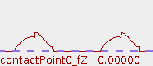
\includegraphics[scale =1.5]{GRF_openloop.pdf} 
  \caption{Ground reaction force when $f_n = 10$}
%  \label{fig.verticalHopper1DOF}
  \end{figure}
  
\end{itemize}
\begin{figure}[H]
\centering
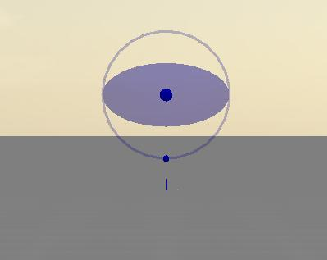
\includegraphics[scale = 0.7]{verticalHopper1DOF.pdf} 
\caption{The vertical hopper, the blue dot at the bottom is the contact point of the massless leg.}
\label{fig.verticalHopper1DOF}
\end{figure}

\begin{figure}[H] 
\centering
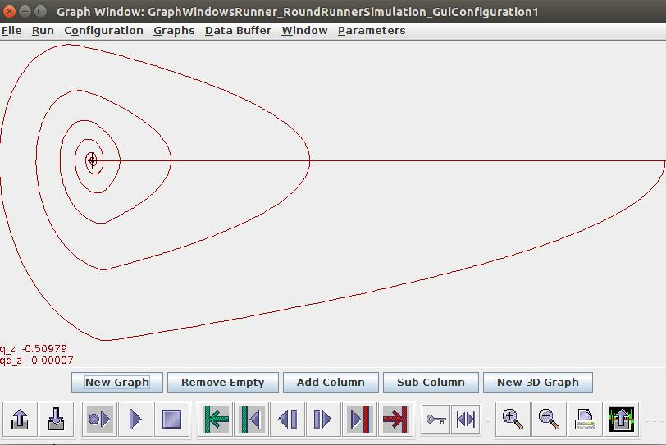
\includegraphics[scale = 0.7]{f1_stable_T0.pdf} 
\caption{Phase portrait (stable spiral) of $f = 1$, period $0$ sec}
%\label{fig.verticalHopper1DOF}
\end{figure}
\begin{figure}[H] 
\centering
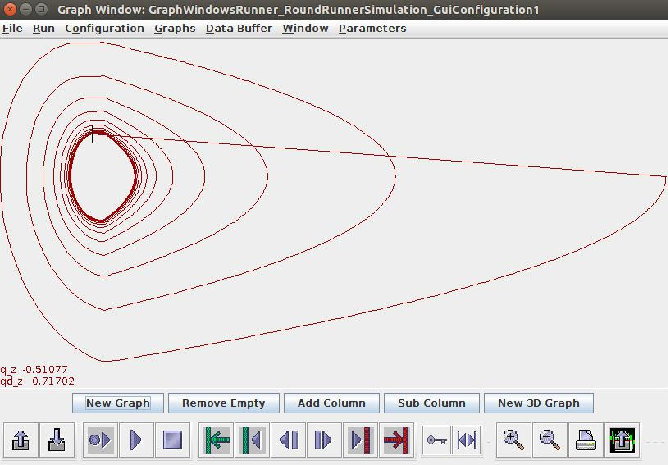
\includegraphics[scale = 0.7]{f10_stable_T0270.pdf} 
\caption{Phase portrait (stable limit cycle) of $f = 10$, period $0.27$sec, (closer to the damped natural period $\approxeq 0.3295$ sec)}
%\label{fig.verticalHopper1DOF}
\end{figure}

\begin{figure}[H]
\centering
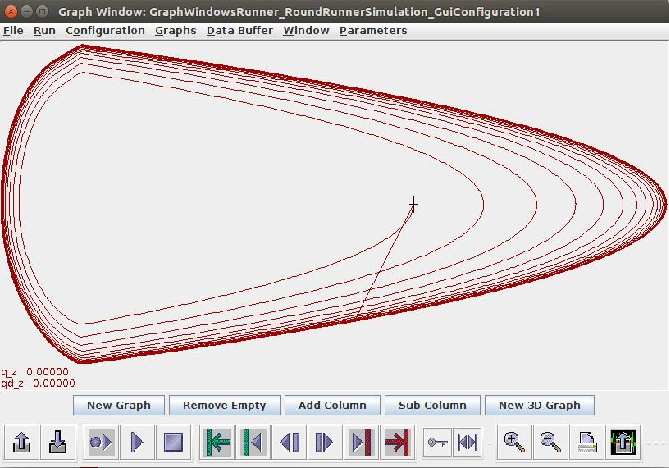
\includegraphics[scale = 0.7]{f50_stable_T0859.pdf} 
\caption{Phase portrait (stable limit cycle) of $f = 50$, period $0.859$ sec}
%\label{fig.verticalHopper1DOF}
\end{figure}

\begin{figure}[H]
\centering
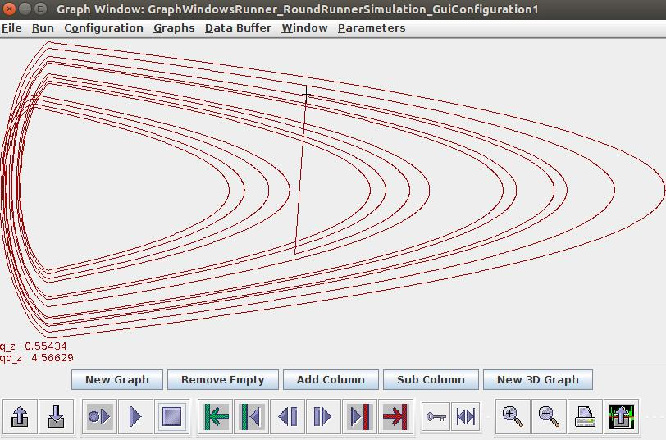
\includegraphics[scale = 0.8]{f100_unstable.pdf} 
\caption{Phase portrait of $f = 100$, no stable limit cycle evolved (might be bifurcation).}
%\label{fig.verticalHopper1DOF}
\end{figure}

\pagebreak

\section{Code implementation}





\subsection{Modeling and Parameters}
Main idea: a virtual wheel (as the massless leg) with radius $r_{wheel}$ penetrate the ground for a distance $r_{pen}$ where a external force point $pe$ is attached on it. A body (with mass $m$ and inertia $Iyy$) is attached to the center of wheel. 
Using PD control to interpret contact force when $p_e$ is under the ground.

\subsubsection*{06/07 First prototype (Not used now)}
\begin{itemize}
\item Joint numbers: 2
\item Joint types: Floating planer joint for virtual wheel and pin joint for the body link.
\item Contact point type: External force point
\item Virtual wheel rotation: set proper initial condition for virtual wheel (also need a large inertia to make it nearly constant).
\end{itemize}

Contact force: Assuming the ground height is $0$,
\begin{align}
F_z &= kp(0-pe_z) + kd(0 - ve_z)\\
\phi &= atan2(pe_x,r_{wheel}-pe_z)\\
F_x &= F_ztan(\phi)
\end{align}
where $ve$ is the velocity vector of the contact point $pe$, $kp$ and $kd$ are the PD control parameters. $F_x$ is calculated so that the vector of ground reaction force $[F_x,F_y,F_z]^T$ will point towards the virtual pivot (the center of the virtual wheel).\\

Assessments:
\begin{itemize}
\item Need to set a non-zero inertia of massless virtual wheel (for numerical stability), otherwise the simulation will diverge.
\item The inertia of virtual wheel need to be a large one for constant rotational speed.
\item Suggestions: remove the massless link, attach the external force point to the body and change its position in the controller every time step.
\end{itemize}

\subsubsection*{06/08 Round Runner}
\begin{itemize}
\item Joint numbers: 1
\item Joint types: Floating planer joint for the body link.
\item Contact point type: External force point
\item Virtual wheel rotation: Assigning the external force point location with respect to the joint in an open loop manner.
\item 
Contact force: Assuming the ground height is $0$,
\begin{align}
F_z &= kp(0-pe_z) + kd(0 - ve_z)\\
\phi &= atan2(pe_x,r_{wheel}-pe_z)\\
F_x &= F_ztan(\phi)
\end{align}
where $ve$ is the velocity vector of the contact point $pe$, $kp$ and $kd$ are the PD control parameters. $F_x$ is calculated so that the vector of ground reaction force $[F_x,F_y,F_z]^T$ will point towards the virtual pivot (the center of the virtual wheel).\\
\end{itemize}



Assessments:
\begin{itemize}
\item The ground reaction force looks better, while the energy is not balanced (after a while it will move towards the negative $x$ direction)
\item The inertia of virtual wheel need to be a large one for constant rotational speed.
\item Suggestions: Use the ground contact point (instead of external force point) to see how it goes.

\end{itemize}

\subsubsection*{06/11 Round Runner(with Ground Contact Point)}
\begin{itemize}
\item Joint numbers: 1
\item Joint types: Floating planer joint for the body link.
\item Contact point type: Ground contact point, linear contact model\footnote[1]{Disable the hardening stiffness in z direction by setting groundStiffeningLength to Double.NEGATIVE\_INFINITY}
\item Virtual wheel rotation: Assigning the external force point location with respect to the joint in an open loop manner.
\item \textbf{Contact point number} Parameterized, currently set to 3-6 points.
\item
Contact force: using built-in functionalities, only assigning the $kp$, $kd$ (PD parameters in the z direction), $kp_x$, and $kd_x$ (PD parameters in the x/y directions).
\end{itemize}



Assessments:
\begin{itemize}
\item Was able to generate a stable walking. Contact point has sliding.
\item Due to setting up stiffness and damping for $x$ and $z$ separately, the force is not always point towards the virtual pivot.

\end{itemize}

\subsubsection*{06/12 Round Runner(with External Contact Point Point)}

\begin{itemize}
\item Implement the same one as 06/11, but replace the ground contact point to the external one (because it is more complex for ground contact point to adjust stiffness/damping as parameters.)
\item implement the linear ground contact model basically.
\end{itemize}


\subsubsection*{06/13 Round Runner}

\begin{itemize}
\item Parameterize contact point numbers
\item Adding enum for switching between different setup: contact point type and the corresponding ground reaction force calculation: (w.r.t to the world frame or inertia frame.)
\end{itemize}
\subsubsection*{06/16 Round Runner (vertical hopper)}

\begin{itemize}
\item Adding vertical hopper with open-loop force control
\item Playing with open-loop force magnitudes for different stability conditions
\end{itemize}
\pagebreak






\section{Info might be useful}

\subsection{Going through references}
\begin{enumerate}
\item Compare different terrestiral locomotions: Some parameters of the walk are not speed- dependent. The swing duration is a constant time parameter \cite{Abourachid2001}.
\item Trunk plays an important role during walking (birds) \cite{Abourachid2011}.
\item The use of these drives (Resonance drives, with adaptive control) allows increasing machine's quickness several times and decreasing energy expenses simultaneously 10-50 times \cite{Akinfiev1999}.
\item Light weight leg (ostrich vs. moa) can run faster\cite{Alexander1985}. Also a famous allometric equation:
\begin{align}
Y = M^{3/4}
\end{align}
where $M$ is the body mass, Y is the metabolic rate.
\item Human's walking may not be really self-optimized: the preferred speed maybe different from the energetically optimal speed\cite{Arnall2012}.
\item It is concluded that the most important adjustment to the body’s spring system to accommodate higher stride frequencies is that leg spring becomes stiffer \cite{Farley1996}.
\item magic equations for imd force (ostrich) \cite{Jindrich2007}
\item gait frequency was reported to be highly correlated with the resonant frequency of the mass-spring model \cite{Lee2013}
\item WABIAN, why you are here? \cite{Lim2008}
\end{enumerate}
\subsection{Categories}

\begin{enumerate}
\item Nonlinear oscillators/components \cite{Akinfiev1999,Anand1966,Babitsky1996,Buchli2006,Chatterjee2012, Karssen2011, Plooij2011};
\item zoology, biomechanics of animals:
\cite{Abourachid2001,Abourachid2011,Alexander1979,Alexander1985,Daley2007}
\item Bio-inspired robots: \cite{Ananthanarayanan2012,Lock2014}
\item Reference I should read: \cite{Cham2002,Daley2006,Kagawa2010,Karssen2011}
\item Article not found (or not free)\cite{Alexander1979}.
\item Robots in 3D: \cite{Coleman1997}
\item Stability analysis (Monocycle, linearized system) \cite{Coleman2010} (Limit cycle) \cite{Cham2002, Kagawa2010} dimensionless \cite{Riese2012}
\item Biology/Anatomical structure \cite{El-Mahdy2010,Gangl2004}
\item Light weight fast robot \cite{Ethington2013,Iida2012}
\item take a look again \cite{Gatesy1991}
\item mechanism design of robot \cite{Grimmer2011}
\item quadruped reference \cite{Hackert2001} MIT Cheetah\cite{Park2012}
\item human energy cost, resonance usage \cite{Holt1991,Arnall2012, Park2013, Racic2009}
\item walking parameterization \cite{Lee2008,Gatesy1991,Weems2006}
\item human-animal differences \cite{Daley2006}
\item open-loop robot \cite{Mombaur2005}, passive robot \cite{Owaki2011, Owaki2010, Owaki2009}
\end{enumerate}
%where x is a vector with n states (i.e. $x\in R^n$) called state variables, u is the control input, y the is control output, and A is a n by n matrix. Depends on the dimension of input and output, the system can be classified as single-input single-output (SISO) system or multi-input multi-output (MIMO) system.\\\\
%Other notes:
% \begin{itemize}
% \item For most of the systems that follow causality, the output has no instantaneous input (i.e. $D=[0]$).
% \item Time-invariant system (don't need to be linear) is also called \emph{autonomous system}. On the other hand, time-varying system is  called \emph{non-autonomous system}.
%\item When B=[0], the system is also called a \emph {unforced system}, as show in Eq \eqref{eqn:unforce}:
%\begin{align}
%\label{eqn:unforce}
%\dot {x}={A}x,
%\end{align}
%\end{itemize} 
%%
%\section{Solution for LTI system}
%\subsection{Laplace transform of a LTI system}
%Assume the initial condition of the state variable $x$ is $x_0$. By applying Laplace transform on both sides of Eq \eqref{eqn:unforce}:
%\[
%sX(s)-x_0=AX(s)\]
%\[\rightarrow(SI-A)X(s)=x_0\]
%\begin{align}
%\label{eqn:LA}
%\rightarrow X(s)=(SI-A)^{-1}x_0,
%\end{align}
%where $I$ is identity matrix. We can derive the Laplace transform  of $x$ : $X(s)$ as shown in Eq\eqref{eqn:LA}. By applying inverse Laplace transform on both sides of Eq\eqref{eqn:LA}, then the solution of LTI system can be derived as follows:
%\[
%\mathscr{L}^{-1}(X(s))=\mathscr{L}^{-1}((SI-A)^{-1}x_0)\]
%\begin{align}
%\label{eqn:sol}
%\rightarrow x(t)=\mathscr{L}^{-1}(\underbrace{(SI-A)^{-1}}_\text{resolvent matrix})x_0=e^{At}x_0
%\end{align}
%
%\subsection{Matrix exponential}
%For a arbitrary constant $a\in R$, $\mathscr{L}^{-1}(s-a)=e^{at}$. Similarly, if $A$ is a square matrix, $\mathscr{L}^{-1}(sI-A)=e^{At}$. The next coming question will be how to evaluate the \emph {matrix exponential} $e^{At}$? One way to go is using Taylor series expansion of the exponential function, which is shown as follows:\\\\
%For $a\in R$ is a constant,
%\[e^{at}=1+at+\frac{1}{2!}a^2t^2+\frac{1}{3!}a^3t^3+\ldots=
%\sum\limits_{k=1}^\infty \frac{1}{k!}a^kt^k\]
%For $A$ is a n by n matrix,
%\[e^{At}=I+At+\frac{1}{2!}A^2t^2+\frac{1}{3!}A^3t^3+\ldots=
%\sum\limits_{k=1}^\infty \frac{1}{k!}A^kt^k\]
%The Taylor series expansion of matrix exponential can also be used for verifying the solution of x:
%\[\dot x=\frac{dx}{dt}=\frac{d}{dt}e^{At}x_0\]
%\[\frac{d}{dt}e^{At}x_0=\frac{d}{dt}(I+At+\frac{1}{2!}A^2t^2+\frac{1}{3!}A^3t^3+\ldots)x_0\]
%\[\frac{d}{dt}e^{At}x_0=(A+A^2t+\frac{1}{2!}A^3t^2+\ldots)x_0\]
%\[\frac{d}{dt}e^{At}x_0=A(I+At+\frac{1}{2!}A^2t^2+\frac{1}{3!}A^3t^3+\ldots)x_0=Ax\]
%Matrix exponential $\Phi(0,t)=e^{At}$ is also called the \emph{state-transition matrix}\\
%(Please refer to: \url{https://en.wikipedia.org/wiki/State-transition_matrix} )
%
%\subsection{Solution of LTI system with control input}
%Considering the following derivative equation:
%\[\frac{d}{dt}(e^{-At}x(t))=-Ae^{-At}x+e^{-At}\dot x\]
%\[=e^{-At}(\dot x-Ax)\]
%\[=e^{-At}(Bu)\]
%Integrate the left hand side from $0$ to $t$:
%\[\int_{0}^{t} \frac{d}{dt}e^{-At}x(t)=[e^{-A\tau}x]_0^t=e^{-At}x(t)-x_0=\int_0^te^{-A\tau}Bu(\tau)d\tau\]
%\[\rightarrow e^{-At}x(t)=x_0+\int_0^te^{-A\tau}Bu(\tau)d\tau\]
%\[\rightarrow x(t)=\underbrace{e^{At}x_0}_\text{homogeneous solution}+\underbrace{\int_0^te^{-A(t-\tau)}Bu(\tau)d\tau}_\text{particular solution}\]
%
%
%\section{Eigenvalues, eigenvectors and system stability}
%\subsection{Eigenvalues and eigenvectors}
%For a matrix $A$, its eigenvalues and eigenvectors can be expressed as follows:
%\begin{align}
%\label{eqn:eigen}
%Av=\lambda v
%\end{align}
%where $\lambda$ is the eigenvalue (a scalar), and v is the eigenvector.
%If $A$ matrix is a n by n full rank matrix, then it will have n eigenvalues with n corresponding eigenvectors.\\\\
%If matrix $A$ is related to the dynamics of a system (e.g. A matrix in Eq \eqref{eqn:LTI}), its eigenvalue and eigenvector usually contain important physical meanings.\\\\
%One interpretation of Eq \eqref{eqn:eigen}: on a specific direction along the eigenvector v, one can use a \emph{scalar} $\lambda$, instead of the system matrix, to describe the system dynamics.
%
%\subsection{Cayley–Hamilton theorem}
%To derive the eigenvalues of a n by n matrix A, one way is to solve the characteristic equation (characteristic polynomial), which is defined as:
%\[det(\lambda I-A)=\lambda^n+a_{n-1}\lambda^{n-1}+\ldots+a_1\lambda+a_0=f(\lambda)=0, \]
%where $I$ is a n by n identity matrix.\\\\
%Cayley–Hamilton theorem states that substituting matrix $A$ for $\lambda$ in the characteristic equation results in the zero matrix, that is,
%\begin{align}
%\label{eqn:CH}
%f(A)=A^n+a_{n-1}A^{n-1}+\ldots+a_1A+a_0I=0
%\end{align}
%By using the equation above, one can utilize it to calculate $A^n$ (i.e. the power of $A$) with reduction of order, or calculate the inverse of matrix $A$ by multiplying $A^{-1}$ on both sides.
%
%\subsection{Similar Transform (Similarity transformation)}
%Definition:  matrices $A$,$B$ $\in R^{n\times n}$, $\exists$ (there exists) $P$ $\in R^{n\times n}$ which is invertible s.t. (such that) $B=PAP^{-1}$\\\\
%Remarks of similar transform
% \begin{itemize}
% \item The eigenvalues of matrices $A$ and $B$ will be the same (i.e. system characteristic is preserved!)
% \item The characteristic equations, ranks, determinants, traces of $A$ and $B$ will also be the same.
% \end{itemize}
%Example:
%A is a n by n matrix with distinct eigenvalues ($\lambda_1\ldots\lambda_n$) and eigenvectors ($v_1\ldots v_n$), then the following equations are satisfied:
%\[Av_1=\lambda_1v_1\]
%\[Av_2=\lambda_2v_2\]
%\[\vdots\]
%\[Av_n=\lambda_1v_n\]
%Those equations can be expressed as the following:
%\begin{align}
%\label{eqn:ST}
%AV=V\Lambda
%\end{align}
%where
%\[V=[v_1,v_2,\ldots,v_n],\]
%\[\Lambda=\left[ \begin{matrix}
%   \lambda_1 &0 &\ldots &\ldots&0 \\
%   0&\lambda_2 & 0&\ldots &0\\
%   \vdots&&\ddots&&\vdots\\
%   0&\ldots&\ldots&0&\lambda_n \end{matrix} \right],\]
%Multiply $V^{-1}$ to the right on both side of Eq \eqref{eqn:ST}, then we can show $\Lambda$ (or the \emph{Jordan form}) is a similar transform of A:
%\[A=V\Lambda V^{-1}\]
%
%\subsection{System stability}
%For a linear system, $\dot x=Ax$ is stable if $Re[\lambda (A)]<0$. In other words, the system is stable if the 
%\emph(zeros) of characteristic equation (i.e. the \emph{poles} of the system) are in the left half plane.
%The criteria above can be used to identify the stability of any linear system. However, this criteria can only works partially for the nonlinear systems. In other words, a more general definition of stability is required for nonlinear system analysis. As a result, Lyapunov proposed other definitions of stability:
%\subsubsection{Lyapunov stability}
%Given a system $\dot x=Ax, x(0)=x_0$, the system is stable if $||x(t)||^2$ is monotonically decrease (i.e. non-increase). Therefore, the condition of Lyapunov stability can be stated as: the system is asymptotically stable if\\
%\[\frac{d}{dt}||x(t)||^2<0\]
%The $||x(t)||^2$ can be expressed as a inner product of vectors (assume x is a colume vector):
%\[\rightarrow \frac{d}{dt}||x(t)||^2=\frac{d}{dt}x^Tx=\dot{x}^Tx+x^T\dot{x}\]
%\[=\dot{x}^TA^Tx+x^TAx\]
%\[=\dot{x}^T(A^T+A)x<0\]
%Example of a stable system: 
%If \[(A^T+A)\leq-vI,\] 
%\[v\geq 0,\]
%where $v \in R$, then the system is asymptotically stable.
%Note:
% \begin{itemize}
% \item Asymptotic stability, which means that the system state will converge to the equilibrium point when $t\rightarrow \infty$
% \item Exponential stability (stronger version) is a form of asymptotic stability, which indicates that the system's convergence will be bounded by a \emph{exponential decay}. Compared to asymptotic stability, exponential stability indicate the minimum rate of decay of the system state response.
% \item For linear systems, all stable systems are guaranteed to be exponentially stable.
% \end{itemize}
%\subsubsection{Quadratic Lyapunov Function}
%Definition of positive definite:
%Given a matrix $P$, P is positive definite (denoted as $P>0$) if $x^TPx>0$ for any $x$ vector except $x$ is a zero vector. Similarly, P is negative definite ($P<0$) if $x^TPx<0$ for any $x$ vector except $x$ is a zero vector.\\
%A more formal version of Lyapunov stability is stated as shown below
%\[x^TPx, P>0,\]
%\[\frac{d}{dt}x^TPx=\dot{x}^TPx+x^TP\dot{x}+x^T\dot{P}x\]
%If system is LTI, then $\dot P=[0]$.
%\[\rightarrow\frac{d}{dt}x^TPx=x^T(A^TP+PA)x\]
%The system is asymptotically stable if the matrix $(A^TP+PA)<0$. \\\\
%Theorem of Lyapunov function (for continuous linear system):
%Given any matrix $Q>0$, $\exists$ unique $P>0$ satisfying $A^TP+PA=-Q$ if and only if the linear system $\dot{x}=Ax$ is globally asymptotically stable. The function $V(x)=x^TPx$ is a Lyapunov function can be used to verify system stability. In addition, the closed form solution of P is availablea as shown:
%\[P=\int_0^\infty e^{A^Tt}Qe^{At}dt\]
%
%\section{Controllability and Observability}
%A system is controllable on $[0,t]$ if given any initial condition, $\exists$ a continuous input $u(t)$ such that $x(t)=0$
%\subsection{Controllability, Controllability Gramian and Controllability Matrix}
%The controllability Gramian is a Gramian used to determine whether or not a linear system is controllable,which is defined as:
%\begin{align}
%\label{eqn:gc}
%\omega(t,0)=\int_0^t\Phi (\tau,0)BB^T\Phi^T(\tau,0)d\tau
%\end{align}
%
%\begin{prop}
%The system is controllable if and only if $\omega(t,0)$ is invertible.
%\end{prop}
%\begin{proof}[Proof of sufficiency]
%If we assume $omega$ is invertible, then we can always define the input as
%\[u=-B^T\Phi^T\omega^{-1}\Phi x_0,\] such that
%\[x(t)=\Phi x_0-\int_0^t\Phi BB^T\Phi^Tw^{-1}\Phi x_0=\Phi x_0-\omega\omega^{-1}\Phi x_0=0\]
%\end{proof}
%
%\begin{prop}
%The system is controllable if and only if the controllability matrix $C_{mat}= \left[ \begin{array}{ccccc} B & AB & A^B & \dots & A^{n-1}B \end{array} \right]$ is full rank.
%\end{prop}
%\begin{proof}[Proof of necessity]
%the controllability Gramian $\omega=\int_0^t\Phi BB^T\Phi d\tau$ can be viewed as the inner product of $\Phi B$: $<\Phi B,\Phi B>=||\Phi B||^2$. Assume $\omega$ is not invertable (i.e. singular), then 
%\[\exists X_a\neq0\] such that \[\omega X_a=0,\]
%where the following equations can thus be derived:
%\[\rightarrow {X_a}^T\omega{X_a}=0\]
%\[\rightarrow ||{X_a}^T\Phi B||=0\]
%\[\rightarrow {X_a}^T\Phi B=0\]
%\begin{align}
%\label{eqn:CM}
%\rightarrow {X_a}^Te^{At} B=0
%\end{align}
%Differentiate Eq \eqref{eqn:CM} about $t$ for $n-1$ times:
%\[{X_a}^Te^{At} AB=0\]
%\[{X_a}^Te^{At} A^2B=0\]
%\[\vdots\]
%\[{X_a}^Te^{At} A^{n-1}B=0\]
%\[\rightarrow {X_a}^Te^{At}\left[ \begin{array}{ccccc} B & AB & A^B & \dots & A^{n-1}B \end{array} \right]={X_a}^Te^{At}C_{mat}=0,\]
%thus $C_{mat}$ is also not invertible(i.e. singular)
%\end{proof}
%\subsection{Observability}
%Observability is a measure for how well internal states of a system can be inferred by knowledge of its external outputs (i.e. If you can measure the output, then you can use it to derive the initial condition of state variables). The observability and controllability of a system are mathematical duals.
%\begin{prop}
%The system is observable if and only if the observability matrix $O_{mat}= \left[ \begin{array}{ccccc} C \\ CA \\ CA^2 \\ \vdots \\CA^{n-1} \end{array} \right]$ is full rank.
%\end{prop}
%\section{Conclusion}
%``I always thought something was %fundamentally wrong with the %universe'' \citep{adams1995hitchhiker}

%\begin{figure}[h!]
%\centering
%\includegraphics[scale=1.7]{universe.jpg}
%\caption{The Universe}
%\label{fig:univerise}
%\end{figure}



\bibliographystyle{plain}
\bibliography{ref}
\end{document}
